% Uncomment this line for on-screen presentation
\documentclass[xcolor={dvipsnames}]{beamer}\usepackage{etoolbox}\newtoggle{printable}\togglefalse{printable}

% Uncomment this line for printable slides (disable animations and don't waste ink)
%\documentclass[handout, xcolor={dvipsnames}]{beamer}\usepackage{etoolbox}\newtoggle{printable}\toggletrue{printable}

% Adjust these for the path of the theme and its graphics, relative to this file
%\usepackage{beamerthemeFalmouthGamesAcademy}
\usepackage{../../beamerthemeFalmouthGamesAcademy}
\graphicspath{ {../../} }

% Default language for code listings
\lstset{language=C++,
		morekeywords={each,in}
}

\begin{document}
\title{Programming Practice VII}   
\subtitle{BSc Computing for Games}

\frame{\titlepage} 

\begin{frame}{Notice}
	
	\begin{itemize}
		\item We will be assessing BA projects most of the day today.
		\item If it is possible, we will pop by the TeachingSpace in the afternoon after assessments have finished.
	\end{itemize}
\end{frame}	

\part{Morning}
\frame{\partpage}

\begin{frame}{Sprint Planning}
	In this session you will:
	
	\begin{itemize}
		\item \textbf{Conduct} a Sprint Planning meeting with your COMP150 group.
		\item \textbf{Prepare} the product backlog on the Trello board.
		\item \textbf{Ensure} that your sprint goal is achievable with the limited time remaining.
		\item \textbf{Strive} for \textit{playability} \textbf{and cut} as many unfinished features as possible that will still allow a playable build to be delivered. 
		\item \textbf{Build} slack-time into your plan to account for code tidying. Remember that 40\% of the available marks are for the sophistication and maintainability of your source code --- read the marking rubric! 
	\end{itemize}
\end{frame}

\part{Afternoon}
\frame{\partpage}

\begin{frame}{Collaborative Project}
	In this session you will:
	
	\begin{itemize}
		\item \textbf{Write} the source code for the collaborative game.
		\begin{itemize}
			\item Remember to update the Trello board and check your code into the shared repository.
			\item Use pair programming where appropriate.
		\end{itemize}
		\item \textbf{Write and update} the team's weekly reports.
		\item\textbf{Prepare} for the Sprint Review and Sprint Retrospective.
		\item \textbf{Complete} the team evaluation, peer evaluations, and self-evaluations.
		\vspace{2ex}
		\item Should you have sufficient time remaining, \textbf{proof read} each others' agile essay.
	\end{itemize}
\end{frame}	

% -------------------------------------------------------

%\part{The compiler}
%\frame{\partpage}
%
%\begin{frame}
%	\frametitle{The build process}
%	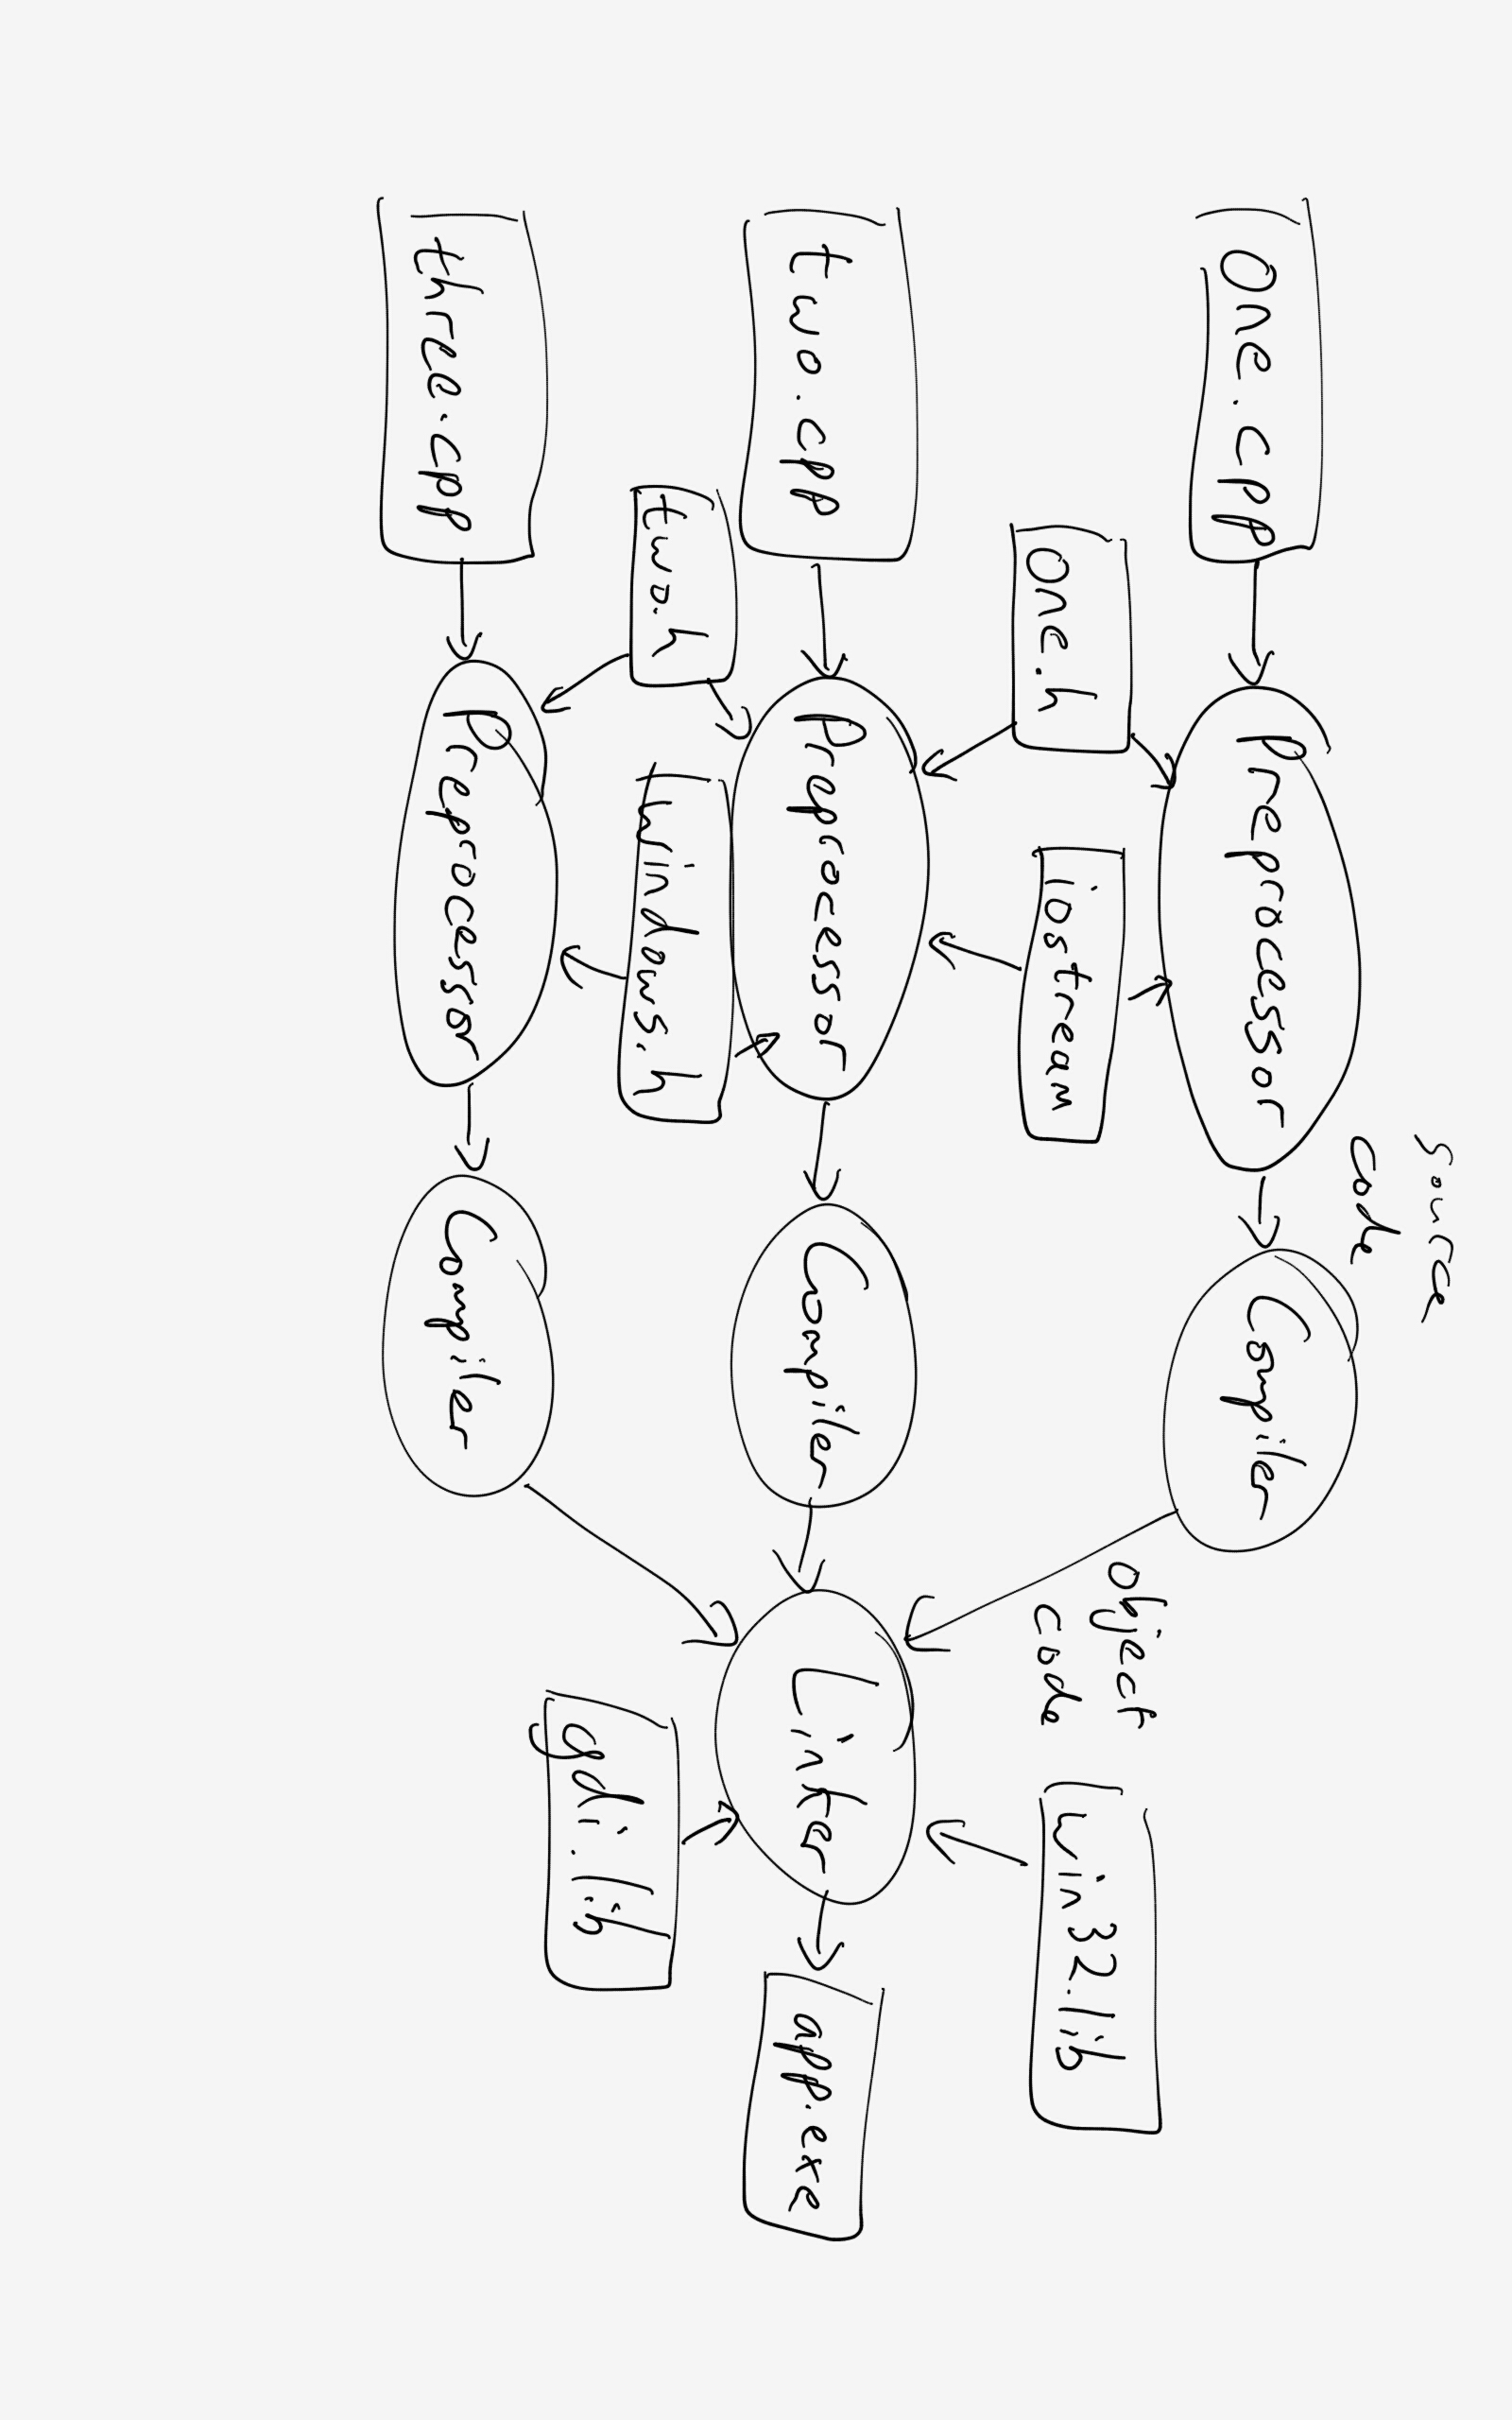
\includegraphics[height=\textwidth,angle=90]{compiler_sketch}
%\end{frame}

\end{document}